\chapter{Ice Reservoirs}

\cleanchapterquote{Glaciers are the secret of life in these otherwise lifeless deserts. But now, they are
melting away at an alarming rate.}{Sonam Wangchuk}{(Ramon Magsaysay awardee, Inventor of ice stupas)}


\section{Introduction}

Irrigation networks in arid mountain regions are completely dependent on the timely availability
of meltwater from glaciers, snow and permafrost \citep{immerzeelImportanceVulnerabilityWorld2020,
farhanHydrologicalRegimesConjunction2015, tveitenGlacierGrowingLocal2007}. With the accelerated decline of
glaciers due to climate change \citep{nusserLocalKnowledgeGlobal2016}, these regions are experiencing acute
water scarcity \citep{norphelSnowWaterHarvesting2015, mukhopadhyayReevaluationSnowmeltGlacial2015}. Further, the
unreliability and the foreseen decrease of seasonal snow cover \citep{chevuturiClimateChangeLeh2018} affects the cryosphere's ability to store water, especially in spring.

For example, due to the short growing period, central Ladakh is a single-cropping area with barley and wheat as
important staples, complemented by vegetables, pulses, and oil seeds
\citep{nusserSociohydrologyArtificialGlaciers2019}. Depending on the altitude, irrigation with complete
flooding of fields (approximately 2-5 cm water column) starts between March and April prior to the melting of
high-altitude glaciers (Fig. \ref{fig:irrigation_cycles}). This results in increased demand during a period of
reduced supply at the onset of the agricultural season (Fig. \ref{fig:irrigation_cycles}).

To cope with this recurrent water scarcity, villagers have developed two types of \ac{AIRs}: ice stupas
and ice terraces (Fig. \ref{fig:AIRforms}). Both the ice reservoirs capture water in the autumn and winter,
allowing it to freeze, and hold it until spring, when it melts and flows down to the fields
\citep{ipccChapterHighMountain2019, vinceGlacierMan2009, clouseLadakhArtificialGlaciers2017,
nusserSociohydrologyArtificialGlaciers2019}. In this way, they retain a previously unused portion of the annual
flow and facilitate its use to supplement the decreased flow during the following spring (Fig.
\ref{fig:irrigation_cycles}).

\begin{figure}[htb]
\centering
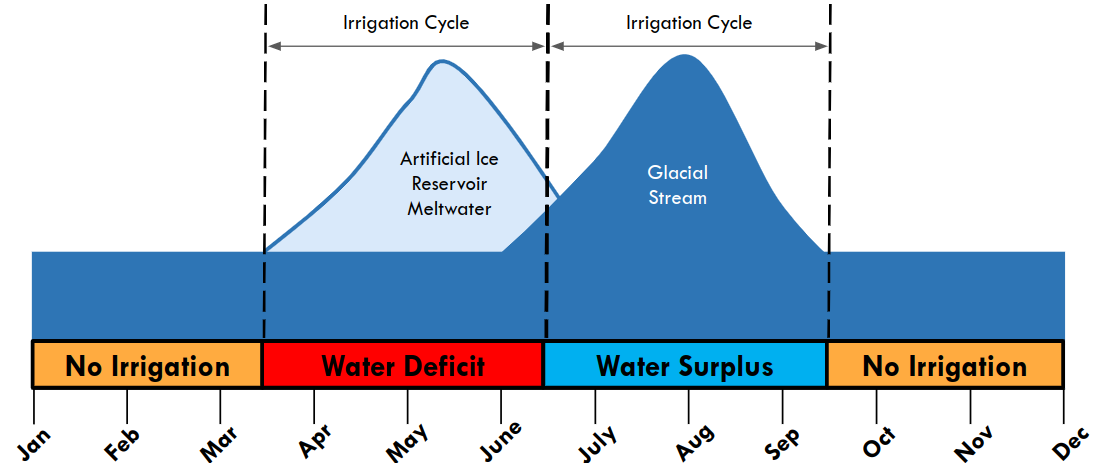
\includegraphics[width=\textwidth]{figs/irrigation_cycles.png}
\caption{Seasonal variation in the availability of irrigation water. The graph highlights the crucial role of
\ac{AIRs} in bridging the gap in water availability. Adapted from \cite{nusserLocalKnowledgeGlobal2016}}
\label{fig:irrigation_cycles}
\end{figure}

\begin{figure}[t]
\centering
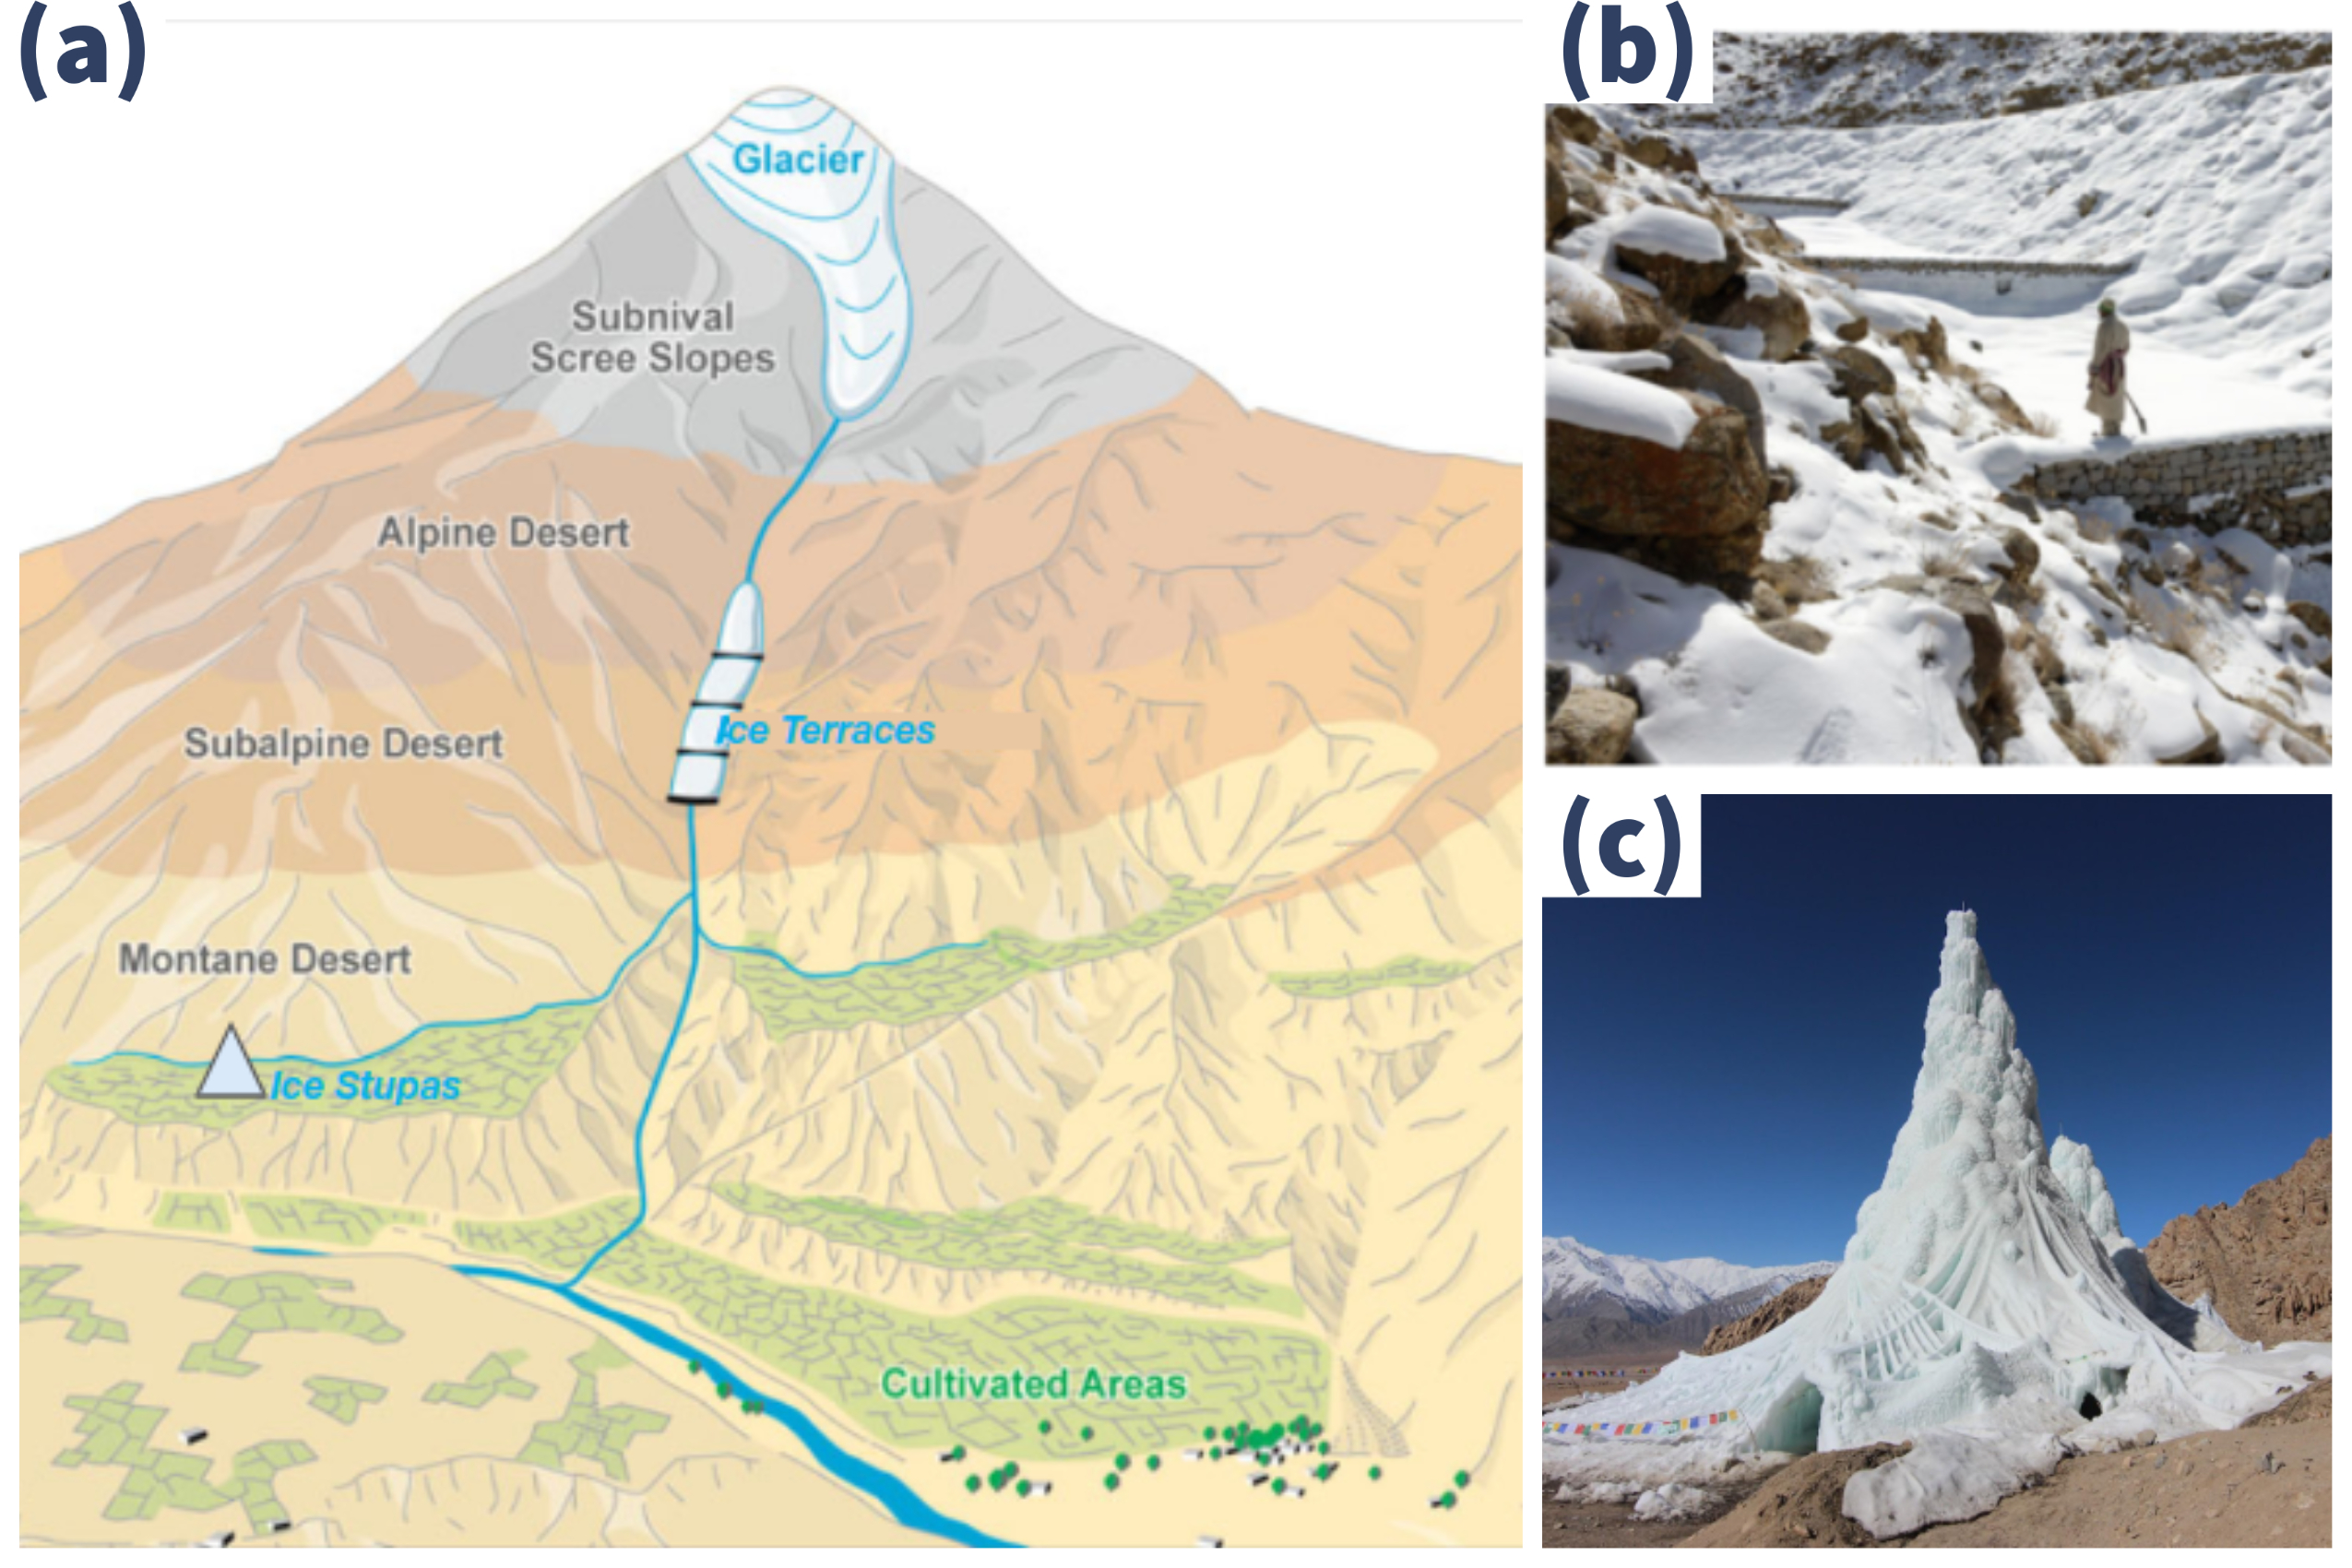
\includegraphics[width=\textwidth]{figs/AIR_forms.jpg}

\caption{(a) Schematic overview of the position of artificial ice reservoirs. These constructions are located at
  altitudes between the glaciers and the irrigation networks in the cultivated areas. (b) Ice terraces at 3900
  m, located above the village of Nang, Ladakh. The cascade is composed of a series of loose masonry walls
  ranging in height from 2 to 3 $m$, which help freeze water for storage. (c) Ice stupas at 3600 m, located
above the village of Phyang, Ladakh. They are made using fountain systems. Adapted from
\cite{nusserLocalKnowledgeGlobal2016}}

\label{fig:AIRforms}
\end{figure}

There is a long tradition of developing such ice harvesting structures in the upper Indus Basin, in both Ladakh,
northern India \citep{labbalTraditionalOasesLadakh2000, nusserIrrigationDevelopmentUpper2012} and various
locations in northern Pakistan \citep{kreutzmannScarcityOpulenceWater2011}. According to oral history and Corona
imagery from 1969, the first ice terraces are older than 50 years. Over the past decade, several ice stupas have
been built to supplement the irrigation water supply of mountain villages in India
\citep{wangchukIceStupaCompetition2020, palmerStoringFrozenWater2022, aggarwalAdaptationClimateChange2021},
Pakistan \citep{awazproductionIceStupaArtificial2022}, Kyrgyzstan \citep{bbcnewsBrightArtificialGlacier2020},
Nepal, and Chile \citep{reutersConservationistsChileAim2021}. In total, more than 500 farmers have constructed
AIRs across 30 villages in the Alps, Andes and Hindu Kush Himalayas.

Despite this widespread adoption, only a few publications examine the role of \ac{AIRs} in the water resource
management of these regions. Notably, none of these prior reports have investigated \ac{AIRs} outside Ladakh.
Moreover, the available estimates of water storage capacity of \ac{AIRs} in Ladakh vary widely
\citep{norphelSnowWaterHarvesting2015, baglaArtificialGlaciersHelp1998}.

Quantifying the water storage capacity of \ac{AIRs} is not straightforward since the processes by which \ac{AIRs} are
formed are complex. These processes are controlled by local topography, meteorology and the construction
strategies used. Modelling approaches to quantifying these processes exist on glacier surfaces but they are not
readily applicable for \ac{AIRs} due to their limited size, and comparatively more variable surface area. Therefore,
conventional glacial modelling approaches need to be adapted in order to capture the
spatio-temporal scale of AIR surface processes. Furthermore, these modelling approaches need to be validated and
calibrated with comprehensive data from field measurements. 

A spirit of improvisation guides the construction of \ac{AIRs} \citep{clouseLadakhArtificialGlaciers2017}.
Depending on the local topography and on how water is supplied, \ac{AIRs} can form as flat sheets
or vertical cones. This has resulted in ice reservoirs exhibiting significant volume variations despite
experiencing similar meteorological conditions. For example, in Ladakh, India, ice terraces have attained volumes up to 30 times
larger than ice stupas \citep{nusserSociohydrologyArtificialGlaciers2019}. However, the
processes driving these differences can only be understood if the complete design methodology behind each construction is available.

This thesis aims to fulfill both these requirements by providing a new set of AIR-specific volume and area
measurements via drone flights, along with meteorological data during the construction period. All these
datasets were generated through construction strategies that used fountain systems. These systems are quantified via in-situ
observations of the fountain characteristics and discharge rate measurements. First, this thesis
formulates a one-dimensional AIR model in order to calibrate and validate it with the procured AIR datasets.
Then it uses this model as a tool to propose a construction strategy that can produce \ac{AIRs}
efficiently and effortlessly. It is important to note that while this thesis reviews published AIR research and
presents a comprehensive quantitative study of their water storage potential, we acknowledge that the farming
communities that have been building these structures since mid-1800s are the custodians of substantial additional knowledge.


\section{Nomenclature and Classification}

By definition, all glaciers, including the smallest ones, are bodies of sedimentary ice which were built
by progressive snow compaction and firnification and flow downhill under the influence of gravity
\citep{benndouglasGlaciersGlaciation2014}. Hence, because of their genesis and composition, \ac{AIRs} differ
from glaciers. Man-made ice structures typically have a lifetime in the order of months and a size million times
smaller than typical glaciers. Therefore, any comparison between these ice structures can be misleading. Since
glaciers are considered natural ice reservoirs, we use the terminology \ac{AIRs} to distinguish the man-made
ice structures described in this thesis from the natural ones. 

However, when classified in terms of size and survival duration, \ac{AIRs} exhibit similar characteristics to
very small glaciers. The glossary of glacier mass balance and related terms by
\citet{cogleyGlossaryGlacierMass2010} defines very small glaciers or glacierets as follows:

\begin{thesis_quotation}
  A very small glacier, typically less than 0.25 $km^2$ in extent, with no marked flow pattern
  visible at the surface. To qualify as a glacieret, an ice body must persist for at least two consecutive
  years. Glacierets can be of any shape, and usually occupy sheltered parts of the landscape. Windborne snow and
  avalanches can be dominant contributors to the accumulation of glacierets.
\end{thesis_quotation}

This rather broad definition of glacierets or very small glaciers may be best suited to describe AIRs, since
they have been measured with areas as high as 0.15 $km^2$ and observed to last beyond a year.

As noted above, AIR's construction strategies are usually inspired by a spirit of improvisation which challenges their
classification. However, it has been found that construction strategies that use fountain systems form conical
\ac{AIRs}, while those that don't form flat sheets of ice. Therefore, this thesis classifies all the \ac{AIRs} produced
based on whether or not they use fountain systems. \ac{AIRs} using fountain systems are called "ice stupas" and those
without are called "ice terraces" as this terminology denotes the resulting shape of the respective \ac{AIRs}
appropriately.

\section{Objectives}

This study employs an integrated approach, which includes field measurements and modelling, to answer the
following research questions: 

\begin{enumerate}

\item What is the influence of construction location and fountain characteristics on ice stupa volume evolution? 

\item How can ice stupa fountain systems be engineered to reduce their water losses and maintenance efforts?

\end{enumerate}

An energy and mass balance model for \ac{AIRs} was designed to answer the first research question
(paper I and III). Since in-situ measurements were required to run this model, we executed a measurement campaign
in Switzerland and India during the past 4 winters. These datasets provided the necessary input, calibration and
validation data to model the evolution of \ac{AIRs} and study their sensitivity to meteorological conditions and
fountain characteristics. 

We also developed new construction strategies to answer the second research question. These
strategies employed fountains the discharge rate of which was regulated by an automation system that used the AIR model
previously developed. Their advantages over traditional construction strategies are quantified in paper II.

\section{Structure}

Chapter 1 introduces the motivation of this work and provides a summary of the state of knowledge about \ac{AIRs}
prior to this thesis. Chapter 2 describes the origins of this technology as a religious practice. Chapter 3
gives an overview about the study sites and introduces the different field techniques applied. The engineering
design of AIR technologies are showcased in Chapter 4 along with suggestions for their improvement. The observed
spatio-temporal variations in AIR volume evolution are presented in Chapter 5 along with suggestions for
choosing future construction locations. Chapter 6 concludes the thesis with a synthesis and the future scope of
this work. Chapter 7 lays out the peer-reviewed work supporting the conclusions of this thesis.
